\chapter{Giới thiệu về mạng nơ-ron nhân tạo}
\label{chp:01}

\section{Lịch sử mạng nơ-ron}
\label{sec:history}
Bước đầu tiên đối với các \textit{mạng nơ-ron} (neural network) đến vào năm 1943 khi Warren McCulloch, một nhà sinh lý học thần kinh và một nhà toán học trẻ, Walter Pitts, đã phát triển các mô hình đầu tiên của mạng nơ-ron. Họ đã viết bài báo \textit{``Tính toán logic của các ý tưởng trong hoạt động thần kinh''} (``The Logical Calculus of the Ideas Immanent in Nervous Activity'') về cách các nơ-ron có thể hoạt động [\ref{refer:1}]. Họ đã mô hình hóa một mạng nơ-ron đơn giản với các \textit{mạch điện} (electrical circuits).

Vào năm 1949, Donald Hebb, một nhà tâm lý học, đã củng cố khái niệm về nơ-ron trong cuốn sách của ông \textit{``Sự tổ chức của hành vi''} (``The Organization of Behavior'') [\ref{refer:2}], một công trình chỉ ra rằng các \textit{lối mòn thần kinh} (neural pathways) được gia cố mỗi khi chúng được sử dụng.

Vào năm 1958, Frank Rosenblatt, một nhà tâm lý học, đã tiến hành một công trình đầu tiên về perceptrons [\ref{refer:3}]. Perceptron là một thiết bị điện tử được chế tạo theo nguyên tắc sinh học và cho thấy khả năng học hỏi. Ông cũng đã viết một cuốn sách trước đó về điện toán thần kinh, \textit{``Nguyên tắc thần kinh học''} (``Principles of Neurodynamics'') [\ref{refer:4}].
Một hệ thống khác là ADALINE (ADAptive LInear Element) được phát triển vào năm 1960 bởi hai kỹ sư điện Bernard Widrow and Marcian Hoff [\ref{refer:5}]. Phương pháp được sử dụng cho việc học khác với phương pháp của Perceptron, nó sử dụng một thuật toán gọi là \textit{trung bình bình phương nhỏ nhất} (least mean square filter - LMS). Máy ADALINE của Widrow và Hoff không chỉ là ``đồ chơi'' mà được dùng thực sự trong các sản phẩm công nghiệp cho đến ngày nay, ví dụ như để lọc đi tiếng ồn trong điện thoại.

Vào năm 1969, Marvin Minsky và Seymour Papert xuất bản một quyển sách về Perceptron ``Perceptrons: An Introduction to Computational Geometry'', trong đó đưa ra nhiều phê phán, và nói rằng những người nghiên cứu Perceptron đã quá lạc quan, vẽ ra một viễn tưởng vể Perceptron mà họ không thể thực hiện được. Minsky và Papert chỉ ra rằng máy Perceptron của Rosenblatt thậm chí không mô phỏng được một số hàm logic cơ bản như là XOR.

Bản thân Minsky và Papert biết rằng, nếu dùng \textit{mạng thần kinh nhân tạo} (artificial neural networks – ANN) với từ hai lớp nơ-ron trở lên (là điều mà các ANN ngày nay có, càng nhiều lớp thì được coi là càng sâu), thay vì chỉ có một lớp nơ-ron như Perceptron, thì giải quyết được vấn đề mô phỏng các hàm logic mà ANN một lớp không mô phỏng được. Tuy nhiên, từ khi quyển sách của Minsky và Papert xuất hiện, việc nghiên cứu ANN bị chững lại trong vòng cả chục năm, cùng với ``mùa đông'' của toàn bộ lĩnh vực \textit{trí tuệ nhân tạo} (Artificial intelligence), ít ai còn dám dùng cụm từ “neural network”. Trong những năm 1970, người ta vẫn dè dặt nghiên cứu ANN, nhưng đội lốt dưới các tên gọi khác, như là \textit{xử lý tín hiện thích nghi} (adaptive signal processing), \textit{nhận dạng 
mẫu} (pattern recognition), \textit{mô hình sinh học} (biological modeling).

Cho đến thập kỉ 1980, nhiều sự kiện diễn ra, gây nên sự quan tâm mới.
Vào năm 1982, John Hopfield đã trình bày một bài báo ``Neural Networks and Physical Systems with Emergent Collective Computational Abilities'' [\ref{refer:6}]. Hopfield mô tả mạng thần kinh nhân tạo tái phát phục vụ như \textit{hệ thống nội dung bộ nhớ địa chỉ} (content-addressable memory system). Các công trình của ông đã thuyết phục hàng trăm nhà khoa học, nhà toán học và nhà công nghệ có trình độ cao tham gia vào lĩnh vực mới nổi của mạng nơ-ron.

Đến năm 1985, \textit{Viện Vật lý Hoa Kỳ} (the American Institute of Physics) đã bắt đầu một cuộc họp thường niên - \textit{``mạng nơ-ron cho máy tính''} (Neural Networks for Computing). Năm 1987, hội nghị mở đầu tiên về mạng nơ-ron trong thời hiện đại; \textit{``Hội nghị quốc tế về mạng nơ-ron''} (IEEE International Conference on Neural Networks) được tổ chức tại San Diego và \textit{``Hiệp hội mạng nơ-ron quốc tế''} (International Neural Network Society - INNS) được thành lập. Năm 1988, tạp chí ``Neural Networks'' được thành lập, tiếp theo đó là ``Neural Computation'' vào năm 1989 và ``IEEE Transactions on Neural Networks'' vào năm 1990.

Những tiến bộ đáng kể đã được thực hiện trong lĩnh vực mạng nơ-ron đủ để thu hút rất nhiều sự chú ý và tài trợ cho nghiên cứu sâu hơn. Ngày nay, các cuộc thảo luận về mạng nơ-ron đang diễn ra ở khắp mọi nơi. Sự tiến bộ vượt ra ngoài các ứng dụng thương mại hiện tại dường như là có thể, và nghiên cứu đang thúc đẩy lĩnh vực này trên nhiều mặt. Các chip dựa trên lý thuyết thần kinh đang nổi lên và ứng dụng cho các vấn đề phức tạp đang phát triển. Rõ ràng, ngày nay là thời kỳ chuyển đổi cho công nghệ mạng thần kinh.

\section{Các thành phần của mạng nơ-ron}
Mạng nơ-ron nhân tạo được lấy cảm hứng và xây dựng nên từ mạng nơ-ron sinh học, vì vậy một mạng nơ-ron nhân tạo cũng bao gồm nhiều nơ-ron đơn lẻ, được gọi là perceptron. Tuy nhiên, để có thể nắm được cách thức hoạt động của một perceptron, trước hết chúng ta cần phải hiểu được một nơ-ron hoạt động như thế nào.

Cấu tạo của một nơ-ron được minh họa bằng hình \ref{fig:structureOfNeuron}. Một nơ-ron sẽ nhận các tín hiệu điện (mức độ mạnh yếu khác nhau) có chứa thông tin từ các \textit{khớp thần kinh} (synapse) của một hay nhiều nơ-ron khác thông qua các \textit{đuôi gai} (dendrit). Các giá trị tín hiệu đầu vào sẽ được tích tụ tại trong \textit{thân nơ-ron} (cell body). Tại đây, nơ-ron sẽ tiến hành thực hiện một quá trình tính toán bao gồm hai bước. 
\begin{itemize}
\item Bước 1, nơ-ron sẽ thực hiện \textit{phép cộng} (summation) để đạt được tổng giá trị các tín hiệu điện. 
\item Bước 2, nơ-ron sẽ so sánh tổng tìm được ở Bước 1 với một \textit{ngưỡng cụ thể} (threshold). 
\end{itemize}
Nếu vượt quá ngưỡng trên, nơ-ron sẽ phát ra một tín hiệu điện, tín hiệu này được truyền qua \textit{sợi trục} (axon) để tới các \textit{khớp thần kinh}. Lúc này, nơ-ron đó được gọi là đang \textit{kích hoạt (activation)}. 

\begin{figure}[h!]
	\centering
		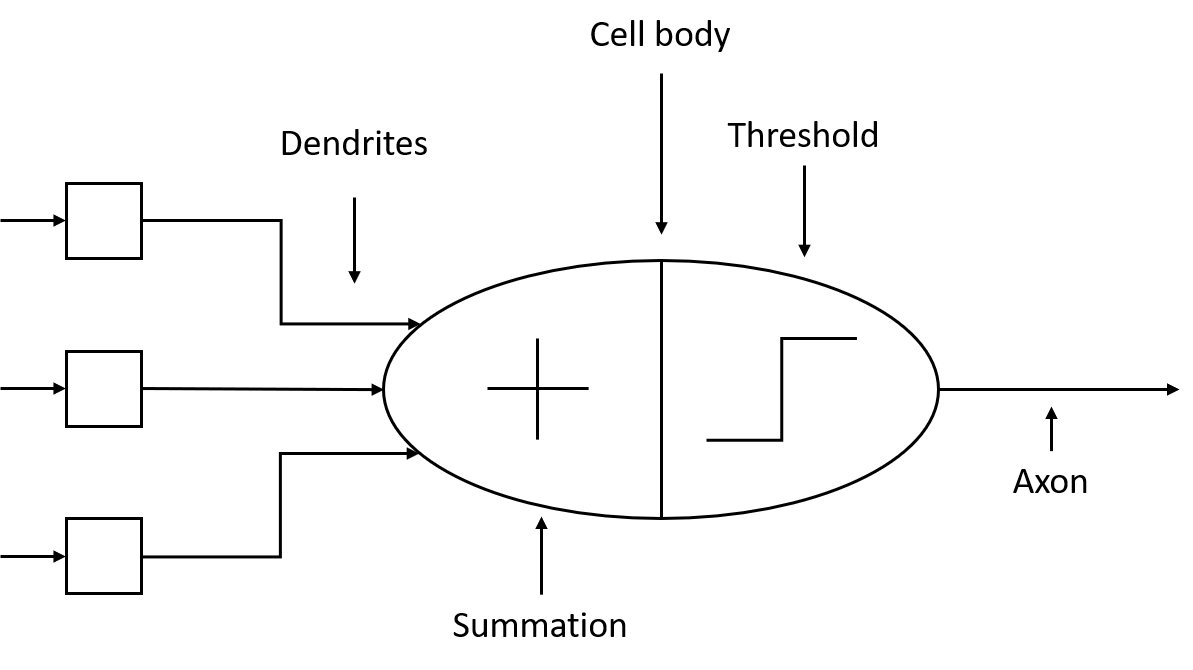
\includegraphics[width=0.5\columnwidth]{chapter01/figure/Picture1.png}
		\centering
	\caption{Hình ảnh minh họa cấu tạo của một nơ-ron sinh học.}
	\label{fig:structureOfNeuron}
\end{figure}

\subsection{Cấu tạo và cách thức hoạt động của một perceptron}
Một nơ-ron nhân tạo (perceptron) được cấu tạo bao gồm các thành phần như hình \ref{fig:structureOfPerceptron}:

\begin{figure}[!h]
	\centering
		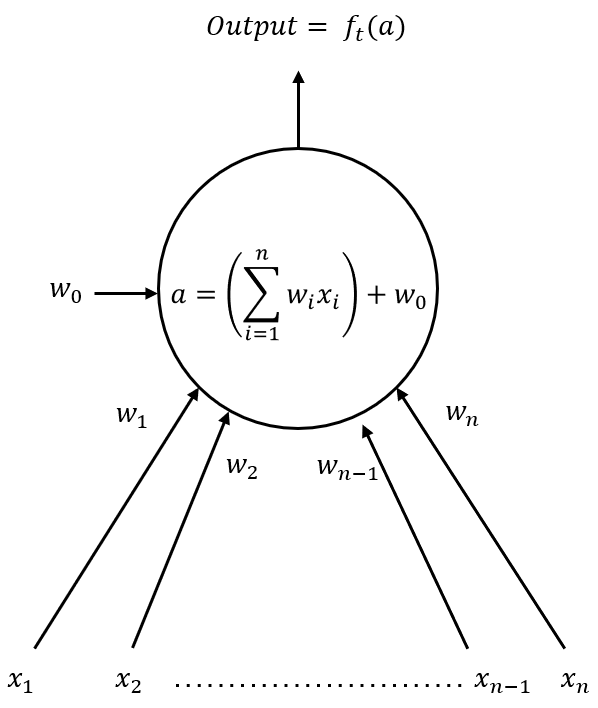
\includegraphics[width=0.4\columnwidth]{chapter01/figure/Picture2.png}
		\centering
	\caption{Hình ảnh minh họa cấu tạo của một perceptron.}
	\label{fig:structureOfPerceptron}
\end{figure}

\noindent Trong đó:
\begin{itemize}
    \item Các giá trị $x_{1},x\textsubscript{2},...,x\textsubscript{n}$ là các tín hiệu đầu vào;
    \item Các giá trị $w\textsubscript{1},w\textsubscript{2},...,w\textsubscript{n}$ là các trọng số của các nhánh tương ứng truyền giá trị $x\textsubscript{1},x\textsubscript{2},...,x\textsubscript{n}$. Giá trị $w\textsubscript{0}$ được gọi là giá trị bias, có thể nhận một giá trị bất kỳ khác 0. Bộ trọng số này là cách để perceptron mô tả độ mạnh yếu của tín hiệu điện trong nơ-ron sinh học;
    \item Giá trị $a$ được tính là $w\textsubscript{0}$ cộng với tổng trọng số của tập tín hiệu đầu vào (tương ứng với bước \textit{summation}). Giá trị a này sẽ được dùng để tính toán hàm kích hoạt $f\textsubscript{t}(a)$;
    \item Kết quả của hàm $f\textsubscript{t}(a)$ sẽ được so sánh với \textit{một ngưỡng (threshsold)} nhằm xác định perceptron có được kích hoạt hay không. Thông thường, giá trị ngưỡng này sẽ được chọn là 0 để tiện trong việc tính toán. Ngoài ra, người ta thường dùng cặp số (1,0) và (1,-1) để đại diện cho trạng thái kích hoạt/không kích hoạt của perceptron;
\end{itemize}
Một điểm lưu ý là perceptron hoạt động dựa trên các phép tính toán số học. Vì vậy, các tín hiệu đầu vào cũng như các trọng số đều cần được biểu diễn dưới dạng các chữ số.

\section{Mạng nơ-ron đa tầng}
\label{sec:MLP}
Có thể thấy rằng, một perceptron đã có thể được coi là một mạng nơ-ron, tính toán kết quả dựa trên tín hiệu đầu vào và kết đầu đầu ra là perceptron đó có được kích hoạt hay không. Trong thực tế, với chỉ một perceptron thì đã có thể giải quyết được bài toán phân loại tuyến tính. Tuy nhiên, đối với các bài toán phức tạp hơn hoặc yêu cầu phân loại phi tuyến (ví dụ như dùng mạng nơ-ron để mô phỏng phép XOR) thì một perceptron không thể đáp ứng được. 
\subsection{Thế nào là mạng nơ-ron đa tầng?}
\label{subsec:whatIsMLP}
Để giải quyết vấn đề trên, chúng ta sử dụng nhiều perceptron được sắp xếp thành các tầng khác nhau. Các perceptron ở tầng sau đều nối tới tầng trước (fully-connected). Một mạng nơ-ron như vậy được gọi là mạng nơ-ron đa tầng.
 
\subsection{Các thành phần của một mạng nơ-ron đa tầng}
\label{subsec:structureOfMLP}
Một mạng nơ-ron đa tầng điển hình thường bao gồm:
\begin{enumerate}
\item Tầng dữ kiện (input layer): Là tầng đầu tiên của mạng,thể hiện các dữ kiện đầu vào;
\item Tầng kết quả (output layer): Là tầng nằm ở vị trí cuối cùng, thể hiện kết quả đầu ra của mạng;
\item Tầng ẩn (hidden layer): Là tầng nằm ở giữa, chịu trách nhiệm trong việc tính toán;
\end{enumerate}

Lưu ý rằng, một mạng nơ-ron đa tầng chỉ có một tầng dữ kiện và một tầng kết quả. Tuy nhiên có thể có một hoặc nhiều tầng ẩn nằm ở giữa, ví dụ như một mạng nơ-ron với hai tầng dưới đây (hình \ref{fig:MLP2HiddenLayer}):

\begin{figure}[h]
	\centering
		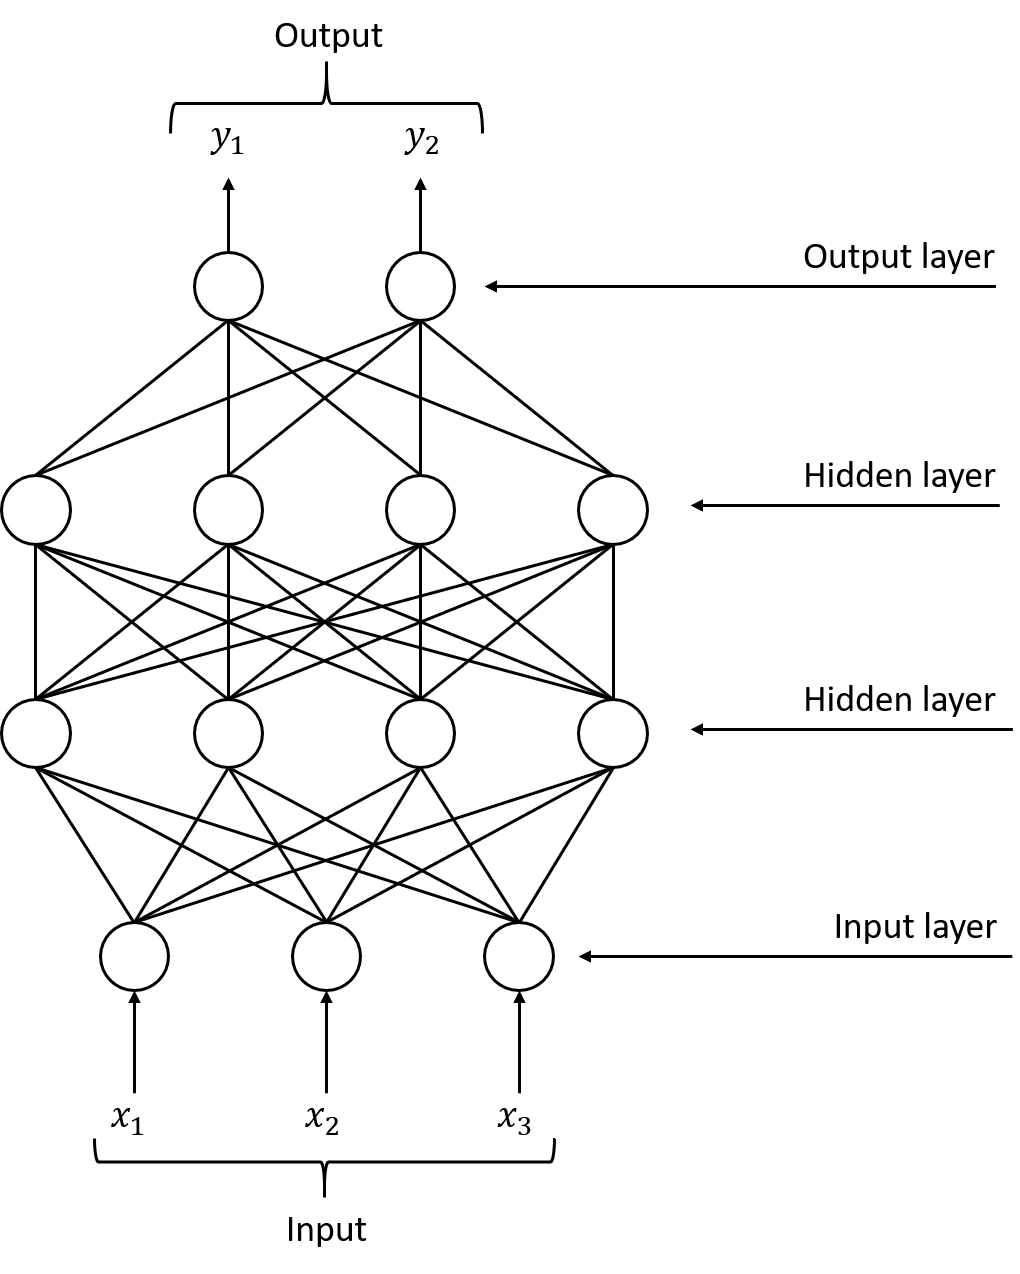
\includegraphics[width=0.5\columnwidth]{chapter01/figure/Picture3.png}
		\centering
	\caption{Hình ảnh mạng nơ-ron đa tầng với 2 tầng ẩn.}
	\label{fig:MLP2HiddenLayer}
\end{figure}

\begin{exmp}
\label{example1}
\hrulefill\\
Cho một mạng nơ-ron ba tầng và các véc-tơ trọng số như hình \ref{fig:example1network} dưới. Với giá trị nào của $x\textsubscript{1}$ và $x\textsubscript{2}$ thì mạng nơ-ron này có kết quả bằng 1?

\begin{figure}[h!]
	\centering
		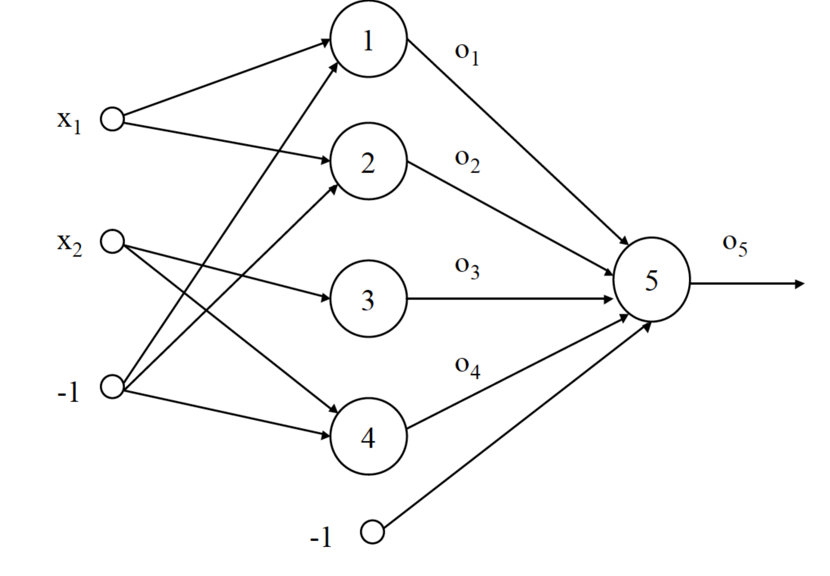
\includegraphics[width=0.7\columnwidth]{chapter01/figure/example 1.png}
		\centering
	\caption{Mạng nơ-ron biểu diễn ví dụ \ref{example1}}
	\label{fig:example1network}
\end{figure}


\noindent Các véc-tơ trọng số có giá trị như sau:

\begin{figure}[h]
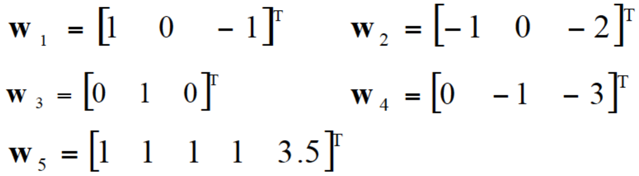
\includegraphics[width=0.6\columnwidth]{chapter01/figure/example 1-weight.png}\
\end{figure}

\noindent Hàm kích hoạt:
\begin{figure}[!h]
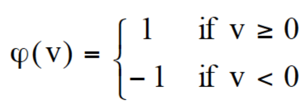
\includegraphics[width=0.3\columnwidth]{chapter01/figure/example 1-activation.png}
\end{figure}

\end{exmp}

\begin{answ}
Chúng ta có thể thấy để thỏa mãn yêu cầu, o\textsubscript{5} phải bằng 1. Điều này dẫn tới nơ-ron số 5 phải được kích hoạt, tương đương với:
\begin{align*} 
&v\textsubscript{5} >= 0 \\ 
\Leftrightarrow &o\textsubscript{1} * 1 + o\textsubscript{2} * 1 + o\textsubscript{3} * 1 + o\textsubscript{4} * 1 + (-1) * 3.5 >= 0
\end{align*}
Như vậy, neural số 1, 2, 3 và 4 phải được kích hoạt để $o\textsubscript{1}, o\textsubscript{2}, o\textsubscript{3}$ và $o\textsubscript{4}$ bằng 1 khiến cho biểu thức trên đúng. Nghĩa là $v\textsubscript{1}, v\textsubscript{2}, v\textsubscript{3}$ và $v\textsubscript{4}$ đều phải lớn hơn hoặc bằng 0. Ta có:
\begin{align}
  &v\textsubscript{1} = x\textsubscript{1} * 1 + x\textsubscript{2} * 0 + (-1) * (-1) = x\textsubscript{1} + 1 \nonumber \\
  \Rightarrow &v\textsubscript{1} >= 0 \Leftrightarrow  x\textsubscript{1} >= -1;  \label{ch1:eq1} \\
  &v\textsubscript{2} = x\textsubscript{1} * (-1) + x\textsubscript{2} * 0 + (-1) * (-2) = -x\textsubscript{1} + 2 \nonumber \\
    \Rightarrow &v\textsubscript{2} >= 0 \Leftrightarrow  x\textsubscript{1} <= 2;  \label{ch1:eq2} \\
  &v\textsubscript{3} = x\textsubscript{1} * 0 + x\textsubscript{2} * (-1) + (-1) * 0 = x\textsubscript{2} \nonumber \\
    \Rightarrow &v\textsubscript{3} >= 0 \Leftrightarrow  x\textsubscript{2} >= 0;  \label{ch1:eq3} \\
  &v\textsubscript{1} = x\textsubscript{1} * 0 + x\textsubscript{2} * (-1) + (-1) * (-3) = -x\textsubscript{2} + 3 \nonumber \\
    \Rightarrow &v\textsubscript{4} >= 0 \Leftrightarrow  x\textsubscript{2} <= 3;  \label{ch1:eq4}
\end{align}
\noindent Từ (\ref{ch1:eq1}), (\ref{ch1:eq2}), (\ref{ch1:eq3}) và (\ref{ch1:eq4}), suy ra để thỏa mãn yêu cầu đã cho thì:
\begin{align*}
-1 <= x\textsubscript{1} <= 2 \And 0 <= x\textsubscript{2} <= 3
\end{align*}
Miền giá trị cần tìm là miền được tô màu đen như hình \ref{fig:example1graph}
\begin{figure}[h]
	\centering
		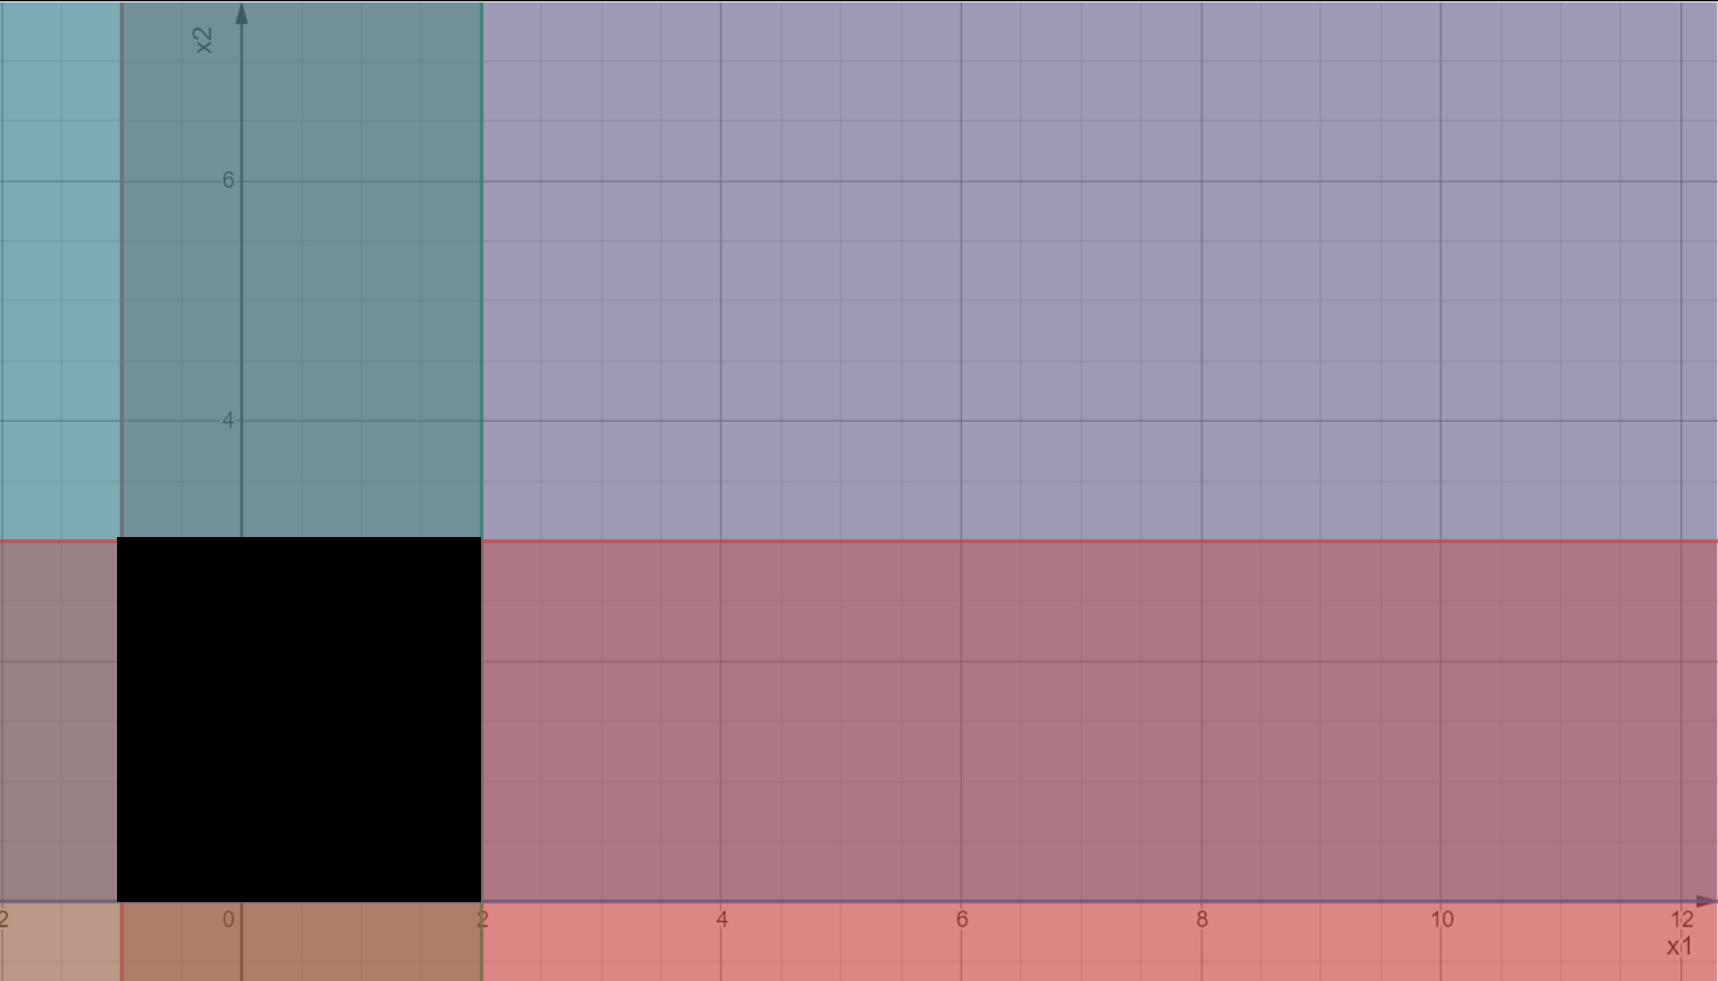
\includegraphics[width=1\columnwidth]{chapter01/figure/example 1_graph.png}
		\centering
	\caption{Miền giá trị cần tìm trong ví dụ \ref{example1}}
	\label{fig:example1graph}
\end{figure}
\end{answ}

\begin{exmp}
\label{example2}
\hrulefill\\
Cho một mạng nơ-ron ba tầng như hình \ref{fig:Example2graph}:

\begin{figure}[h]
	\centering
		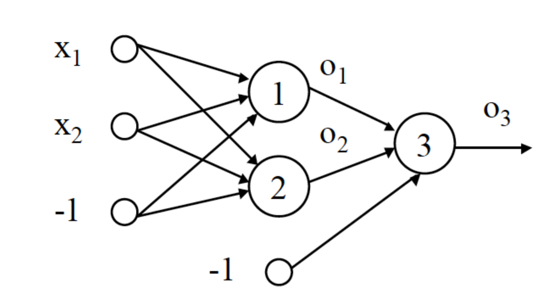
\includegraphics[width=0.7\columnwidth]{chapter01/figure/example 2.png}
		\centering
	\caption{Mạng nơ-ron biểu diễn ví dụ \ref{example2}}
	\label{fig:Example2graph}
\end{figure}

\noindent Các véc-tơ trọng số có giá trị như sau:

\begin{figure}[h]
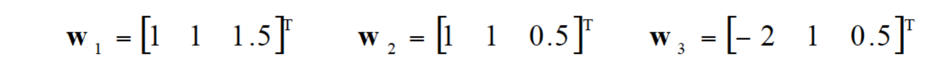
\includegraphics[width=1\columnwidth]{chapter01/figure/example 2-weight .png}
\end{figure}

\noindent Giả sử rằng:

\begin{figure}[!h]
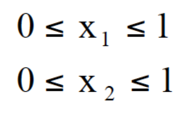
\includegraphics[width=0.2\columnwidth]{chapter01/figure/example 2-assume.png}
\end{figure}

\noindent Với giá trị nào của x\textsubscript{1} và x\textsubscript{2} thì mạng nơ-ron này có kết quả là 1 với hàm kích hoạt như sau:
\begin{figure}[!h]
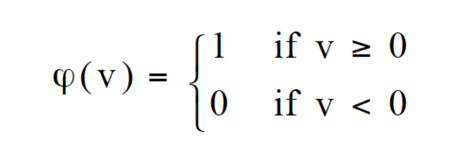
\includegraphics[width=0.4\columnwidth]{chapter01/figure/example 2-activation.png}
\end{figure}
\end{exmp}

\begin{answ}
Tương tự như ví dụ trên, ta có thể thấy rằng:
\begin{align}
  &o\textsubscript{3} = 1 \nonumber \\
  \Leftrightarrow  &o\textsubscript{1} * (-2) + o\textsubscript{2} * 1 + (-1)* 0.5 >= 0 \nonumber \\
  \Leftrightarrow  &-2o\textsubscript{1} + o\textsubscript{2} - 0.5 >= 0 \nonumber
\end{align}
Do o\textsubscript{1} và o\textsubscript{2} chỉ nhận giá trị là 0 hoặc 1. Nên để thỏa mãn biểu thức trên, ta có:
\(o\textsubscript{1} = 0\) và \(o\textsubscript{1} = 1\), trong khi đó:
\begin{align}
  &o\textsubscript{1} = 0 \nonumber\\
  \Leftrightarrow &v\textsubscript{1} = x\textsubscript{1} * 1 + x\textsubscript{2} * 1 + (-1) * 1.5 = x\textsubscript{1} + x\textsubscript{2} - 1.5 < 0 \nonumber\\
  \Rightarrow &x\textsubscript{1} + x\textsubscript{2} < 1.5 \label{eqn:eq2_1}\\
  &o\textsubscript{2} = 1 \nonumber\\
  \Leftrightarrow &v\textsubscript{2} = x\textsubscript{1} * 1 + x\textsubscript{2} * 1 + (-1) * 0.5 = x\textsubscript{1} + x\textsubscript{2} - 0.5 >= 0 \nonumber\\
  \Rightarrow &x\textsubscript{1} + x\textsubscript{2} >= 0.5 \label{eqn:eq2_2}
\end{align}
\noindent Từ \ref{eqn:eq2_1} và \ref{eqn:eq2_2} suy ra kết quả cần tìm: \( 0.5 <= x\textsubscript{1} + x\textsubscript{2} < 1.5\)\\

\noindent Như vậy, kết quả cần tìm là cặp giá trị x\textsubscript{1} và x\textsubscript{2} sao cho điều kiện trên thỏa mãn. Một điểm đặc biệt là nếu như x\textsubscript{1} và x\textsubscript{2} chỉ nhận giá trị 0 và 1 thì mạng nơ-ron này có thể áp dụng để biểu diễn phép toán luận lý XOR (tham khảo Bảng dự thật dưới đây).

\begin{figure}[h]
	\centering
		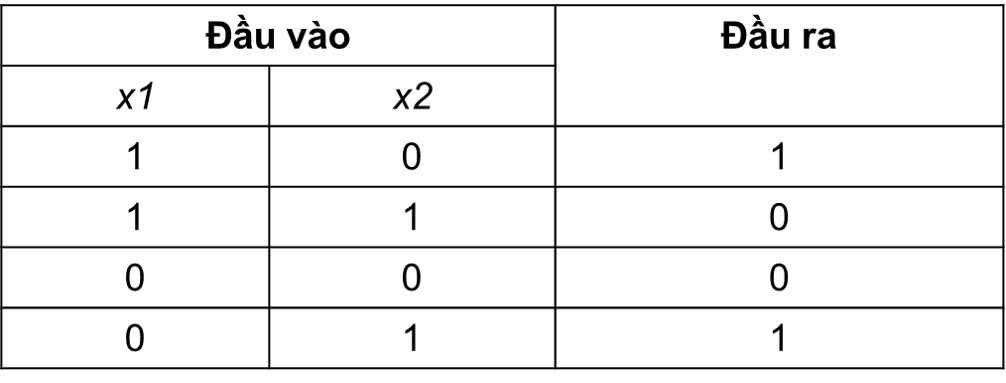
\includegraphics[width=0.6\columnwidth]{chapter01/figure/bang su that XOR.png}
		\centering
	\caption{Bảng sự thật biểu diễn phép XOR trong ví dụ \ref{example2}}
\end{figure}
\end{answ}

\section{Sử dụng neural network cho bài toán phân loại}
\label{sec:classification}
Một trong những ứng dụng quan trọng của mạng nơ-ron là sử dụng cho bài toán phân loại. Đối với bài toán phân loại tuyến tính thì chỉ cần xây dựng mạng nơ-ron với một perceptron. Xét ví dụ sau:

\begin{exmp}
\label{example3}
\hrulefill\\
Xem xét bài toán trong thực tế như sau: Một trường chuyên tổ chức thi để tuyển sinh năm học mới, bao gồm hai môn Toán và Văn, trong đó Toán nhân hệ số 2. Để có thể đậu, học sinh cần phải có tổng điểm xét tuyển lớn hơn hoặc bằng 21. 

Hãy xây dựng một mạng nơ-ron để phân loại học sinh, trong đó điểm Toán được ký hiệu là x, điểm Văn được ký hiệu là y. Kết quả của mạng là 0 hoặc 1, tương đương với học sinh đó đậu hoặc rớt.
\end{exmp}
\begin{answ}
Theo yêu cầu bài toán, ta cần xây dựng mạng nơ-ron dựa trên biểu thức sau:
\begin{align*}
  &2x + y >= 21 \\
  \Leftrightarrow &2x + y -21 >= 0
\end{align*}
Như vậy, khi chuyển sang biểu diễn dưới dạng một mạng nơ-ron, ta có tập giá trị đầu vào là một véc-tơ [x,y,1] và tập trọng số tương ứng có giá trị là [2,1,-21], với \(w\textsubscript{0} = -21\) (trọng số bias tùy ý khác 0). 

\begin{figure}[h]
	\centering
		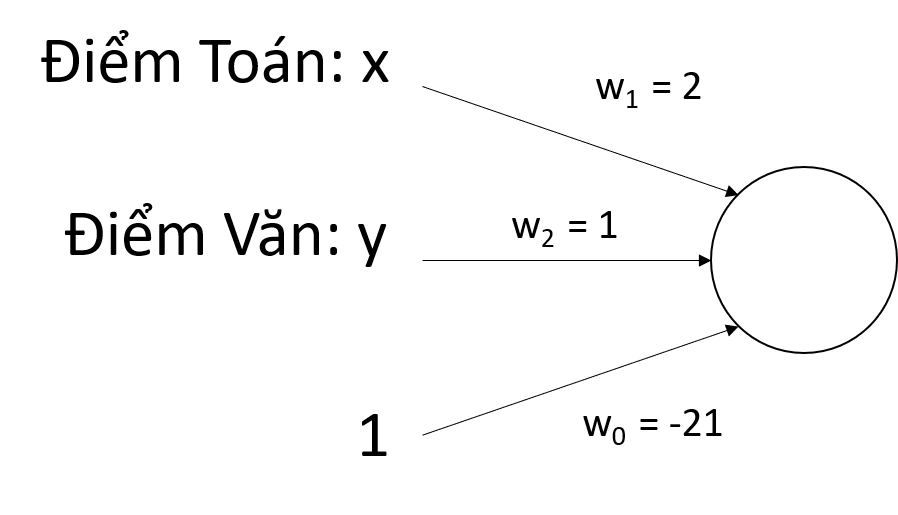
\includegraphics[width=0.5\columnwidth]{chapter01/figure/example 3.png}
        \caption{Mạng nơ-ron biểu diễn ví dụ \ref{example3}}
		\centering
\end{figure}

Ta có, tổng trọng số \(a = 2x + y - 21\). Mạng nơ-ron này chỉ được kích hoạt (tương đương với học sinh đó thỏa mãn điều kiện đậu) khi và chỉ khi \(a >= 0\), tương ứng với vùng màu xanh dương trong biểu đồ \ref{fig:example3-miengiatri}.

\begin{figure}[!h]
	\centering
		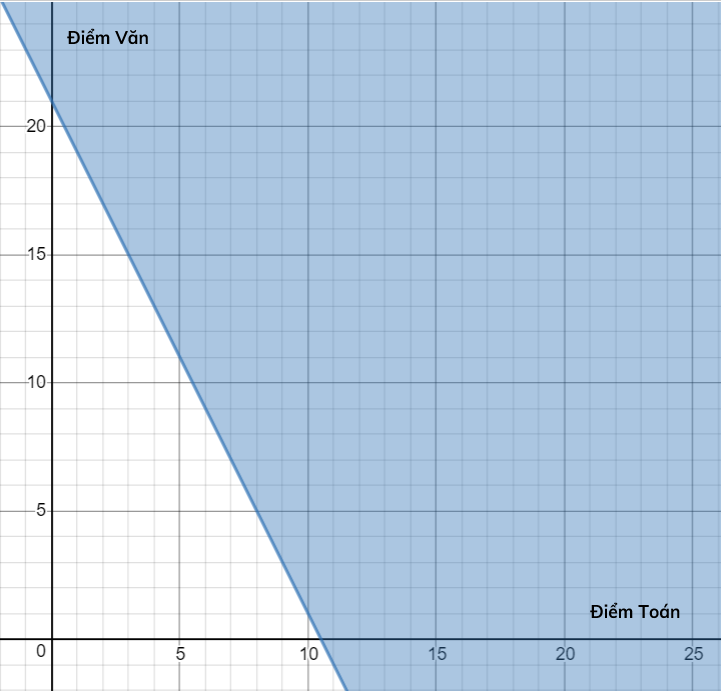
\includegraphics[width=0.55\columnwidth]{chapter01/figure/example 3 - graph 1.PNG}
        \caption{Miền giá trị thỏa mãn yêu cầu đề bài}
        \label{fig:example3-miengiatri}
		\centering
\end{figure}

Tuy nhiên, thực tế điểm Toán và điểm Văn luôn nhận giá trị là số dương \(<= 10\). Khi gán thêm điều kiện này, ta có kết quả là miền giá trị được tô màu đen trong đồ thị \ref{fig:example3-miengiatri2}.

\begin{figure}[h!]
	\centering
		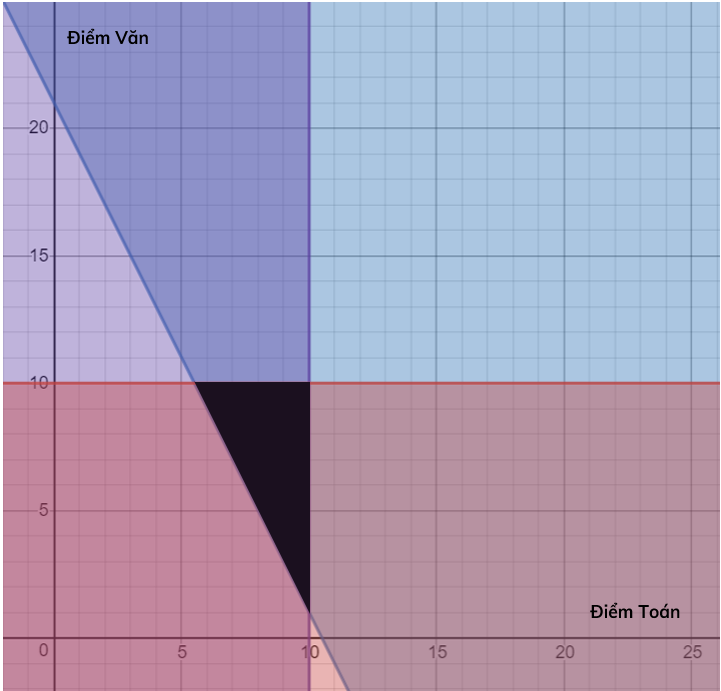
\includegraphics[width=0.55\columnwidth]{chapter01/figure/example 3 - graph 2.PNG}
        \caption{Miền giá trị thỏa mãn yêu cầu đề bài sau khi ràng buộc về khoảng giá trị của điểm Toán và điểm Văn}
        \label{fig:example3-miengiatri2}
		\centering
\end{figure}

Cần lưu ý rằng trọng số bias phải khác 0 để tránh trường hợp phương trình tổng trọng số a được biểu diễn bởi một đường thẳng đi qua gốc tọa độ O(0,0). Điều này dẫn tới khi huấn luyện mạng nơ-ron, thì các kết quả mà mạng này học được chỉ xoay quanh gốc tọa độ O, không đảm bảo tính tổng quát để áp dụng cho các bài toán trong thực tiễn.
\end{answ}
Ví dụ trên đã sử dụng mạng nơ-ron với một perceptron để phân loại bài toán tuyến tính (như hình \ref{fig:neuronRegion}.a bên dưới). Tuy nhiên, đối với bài toán phi tuyến (như các hình \ref{fig:neuronRegion}.b, c, d) thì cần phải xây dựng mạng nơ-ron ba tầng.

\begin{figure}[!h]
	\centering
		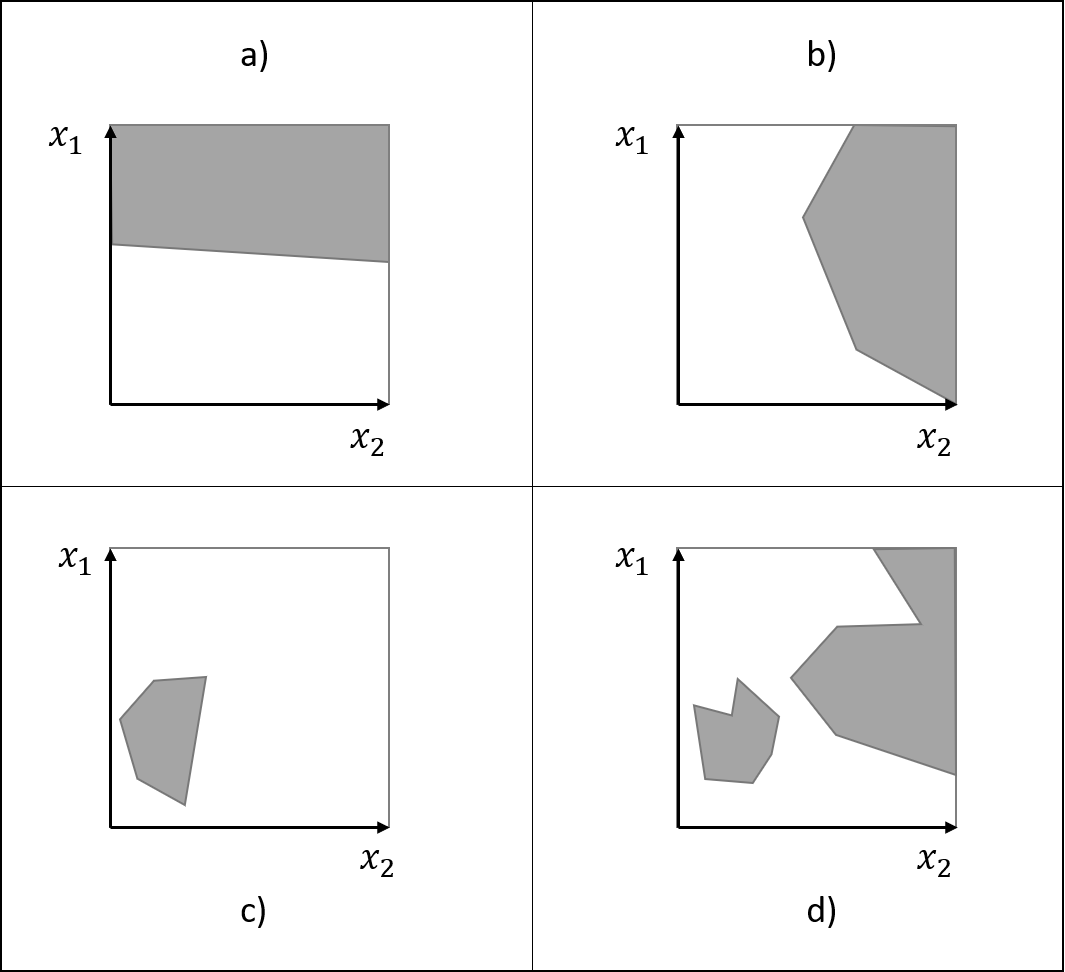
\includegraphics[width=0.6\columnwidth]{chapter01/figure/Picture4.png}
    	\caption{Sử dụng mạng nơ-ron ba tầng để biểu diễn các miền giá trị phi tuyến}
	\centering
	\label{fig:neuronRegion}
\end{figure}

Trong đó, tầng đầu tiên (tầng dữ kiện) sẽ chia đồ thị thành hai nửa bởi một đường thẳng. Tầng thứ hai (tầng ẩn) sẽ hình thành các miền giá trị cần tìm bằng cách kết hợp các phép toán luận lý (AND, OR và NOT) trên nửa đồ thị đã được phân chia của tầng đầu tiên. Bằng cách tăng số lượng tầng ẩn, mạng nơ-ron thậm chí có thể biểu diễn gần đúng các hình tròn thông qua một tập các đường thẳng, ví dụ như hình \ref{fig:circleNeuron}

\begin{figure}[!h]
	\centering
		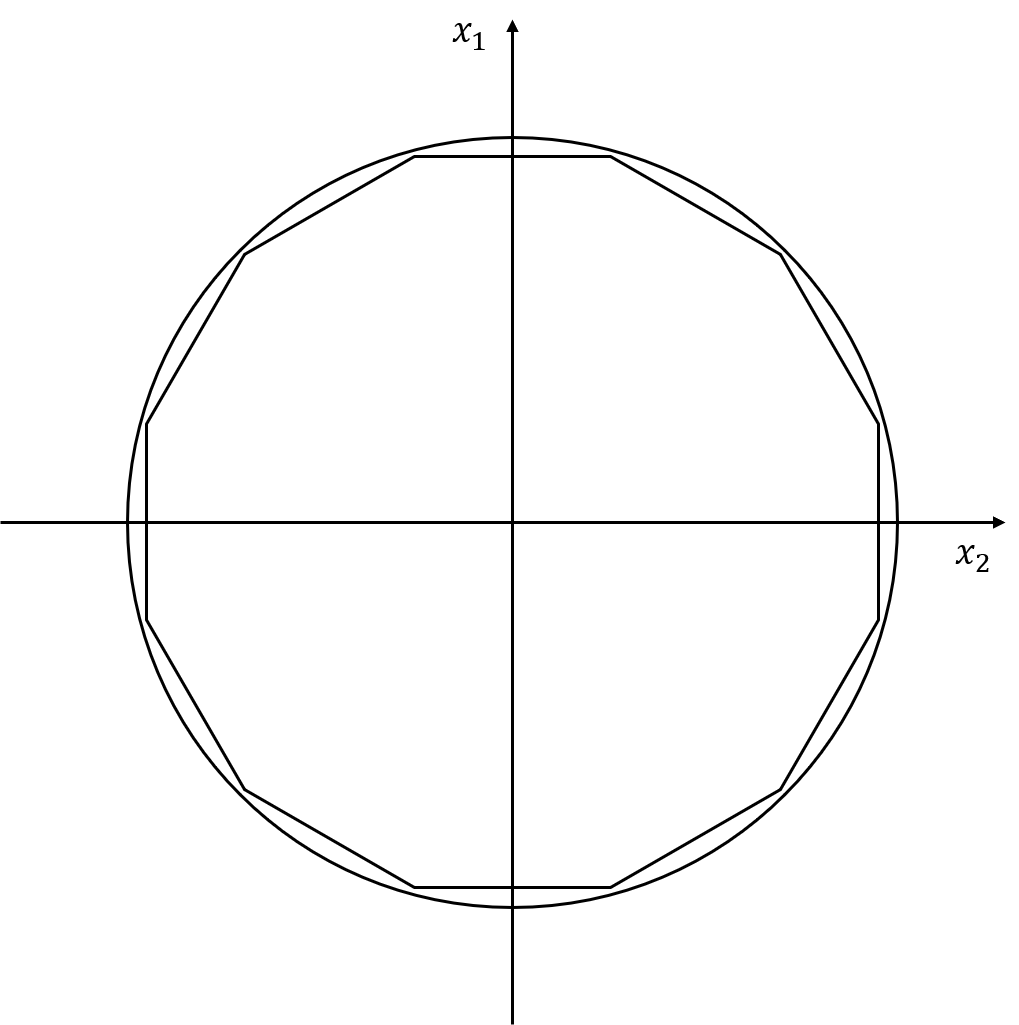
\includegraphics[width=0.5\columnwidth]{chapter01/figure/Picture5.png}
    	\caption{Sử dụng mạng nơ-ron để biển diễn gần đúng miền giá trị là hình tròn}
	\centering
	\label{fig:circleNeuron}
\end{figure}

\section{Kết chương}
\label{sec:endChp}

Chúng ta có thể thấy rằng, mạng nơ-ron được biểu diễn toàn bộ bằng các phép toán số học. Vì vậy, nếu tìm được các bộ trọng số phù hợp với từng bài toán phân loại thì ta hoàn toàn có thể áp dụng mạng nơ-ron một cách hiệu quả, nhanh chóng bằng cách cấu hình sẵn phần cứng với các trọng số cần thiết. 

Tuy nhiên, trong thực tế thì việc để tìm được các bộ trọng số không dễ dàng, đặc biệt là đối với những bài toán phức tạp và cần mô hình bởi mạng nơ-ron đa tầng với nhiều tầng ẩn và nhiều perceptron. Để giải quyết vấn đề này, các nhà khoa học đã tìm ra được phương pháp huấn luyện mạng nơ-ron để có thể tìm ra bộ trọng số tối ưu, vấn đề này sẽ được trình bày trong chương tiếp theo.

\newpage

\section{Bài tập}

\begin{exer}
\label{chp01:exer1}
Cho một mạng nơ-ron ba tầng và các véc-tơ trọng số như hình \ref{fig:exercise1}. Với giá trị nào của x\textsubscript{1} và x\textsubscript{2} thì mạng nơ-ron này có kết quả bằng 1? Vẽ biểu đồ minh họa.
\begin{figure}[!h]
	\centering
		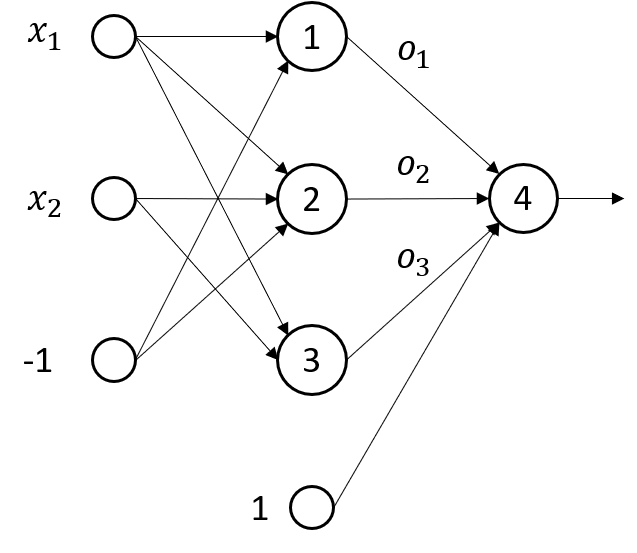
\includegraphics[width=0.5\columnwidth]{chapter01/figure/excercise-1.png}
    	\caption{Mạng nơ-ron trong bài tập \ref{chp01:exer1}}
	\centering
	\label{fig:exercise1}
\end{figure}

Các véc-tơ trọng số có giá trị như sau:
\begin{align*}
w\textsubscript{1} = [2,0,1] \textsuperscript{T} \quad w\textsubscript{2} = [1,2,1] \textsuperscript{T} \quad w\textsubscript{3} = [1,3,0] \textsuperscript{T} \quad w\textsubscript{4} = [2,3,1] \textsuperscript{T} \quad
\end{align*}

Hàm kích hoạt
\begin{align*}
        \varphi (v) = \left\{ \begin{array}{ll}
        1 & \mbox{nếu $v \geq 0$};\\
        0 & \mbox{nếu $v < 0$}.\end{array} \right.
\end{align*}
\end{exer}

\begin{exer}
\label{chp01:exer2}
Thiết kế một mạng nơ-ron để chọn ra các sinh viên toàn diện. Tiêu chí để chọn bao gồm điểm trung bình (số nguyên dương), hạnh kiểm (bao gồm các mức 0-Yếu, 1-Trung Bình, 2-Khá, 3-Giỏi) và điểm rèn luyện (thấp nhất là 0 điểm và cao nhất là 10 điểm). Xét biểu thức sau:\\
\\
\textit{Điểm danh hiệu =  điểm trung bình x 2 + điểm hạnh kiểm + điểm rèn luyện;}\\
\\
\noindent Sinh viên sẽ được nhận danh hiệu toàn diện nếu như \textit{điểm danh hiệu} lớn hơn hoặc bằng 24.
\end{exer}

\begin{exer}
Trong bài tập \ref{chp01:exer2}, nếu như thay đổi  bias đã chọn ban đầu thành một giá trị khác (tùy chọn), thì tập trọng số sẽ cần thay đổi như thế nào?
\end{exer}

\begin{exer}
Trong bài tập \ref{chp01:exer1}, nếu như thay đổi giá trị bias ở tầng thứ 2 từ 1 sang -1. Thì miền giá trị x\textsubscript{1} và x\textsubscript{2} cần tìm có thay đổi không? Vẽ lại biểu đồ minh họa cho trường hợp này và so sánh với trường hợp ban đầu.
\end{exer}